\begin{center}
\Huge
	Trekanter
\end{center}

\subsection*{Ensvinklede trekanter}
\stepcounter{section}

Vi lægger dette afsnit ud med at genopfriske nogle begreber fra grundskolen. Vi begynder med at definere, hvad der menes med \textit{ligedannede} eller \textit{ensvinklede} trekanter. 
\begin{defn}
	To trekanter $\triangle ABC$ og $\triangle PQR$ siges at være \textit{ligedannede} eller \textit{ensvinklede}, hvis
	vinklerne parvist opfylder at være ens i de to trekanter. Mere præcist, at vinklerne opfylder
	\begin{align*}
		&\angle A = \angle P, & &\angle B = \angle Q, & &\angle C = \angle R. 
	\end{align*}
\end{defn}
På Figur \ref{fig:ensvinklede} kan vi se to ensvinklede trekanter
\begin{figure}[H]
	\centering
	\begin{tikzpicture}
		%Trekant1
		\draw[color = olive, thick] (0,0) -- (2*2,0)
		node[midway, anchor = north] {$c$};
		\draw[color = olive, thick] (0,0) -- (1.4*2,1*2)
		node[midway, anchor = south east] {$b$};
		\draw[color = olive, thick] (1.4*2,1*2) -- (2*2,0)
		node[midway, anchor = south west] {$a$};
		\node[color = olive, anchor = east] at (0,0) {$A$};
		\node[color = olive, anchor = west] at (2*2,0) {$B$};
		\node[color = olive, anchor = south] at (1.4*2,1*2) {$C$};
		%VinkelA
		\draw[color = olive, thick] (0+0.4,0) arc (0:35.54:0.4); 
		%VinkelB
		\draw[color = olive, thick] (4-0.5,0) arc (180:180-59.04:0.5); 
		\draw[color = olive, thick] (4-0.4,0) arc (180:180-59.04:0.4); 
		%Trekant2
		\draw[color = olive, thick] (3*2,0) -- (6*2,0)
		node[midway, anchor = north] {$r$};
		\draw[color = olive, thick] (3*2,0) -- (5.1*2,1.5*2)
		node[midway, anchor = south east] {$q$};
		\draw[color = olive, thick] (5.1*2,1.5*2) -- (6*2,0)
		node[midway, anchor = south west] {$p$};
		\node[color = olive, anchor = east] at (3*2,0) {$P$};
		\node[color = olive, anchor = west] at (6*2,0) {$Q$};
		\node[color = olive, anchor = south] at (5.1*2,1.5*2) {$R$};
		%VinkelA
		\draw[color = olive, thick] (6+0.4,0) arc (0:35.54:0.4); 
		%VinkelB
		\draw[color = olive, thick] (6*2-0.5,0) arc (180:180-59.04:0.5); 
		\draw[color = olive, thick] (6*2-0.4,0) arc (180:180-59.04:0.4); 
	\end{tikzpicture}
	\caption{To ensvinklede trekanter $\triangle ABC$ og $\triangle PQR$.}
	\label{fig:ensvinklede}
\end{figure}

For ensvinklede trekanter gælder der, at forholdet mellem sidelængderne i trekanterne er konstant. Før vi formulerer dette som en sætning, så betragter vi et eksempel
\begin{exa}
	Vi betragter de to ensvinklede trekanter $\triangle ABC$ og $\triangle PQR$, der ses på
	 Figur \ref{fig:ensvinkledeExa}. 
	\begin{figure}[H]
		\centering
		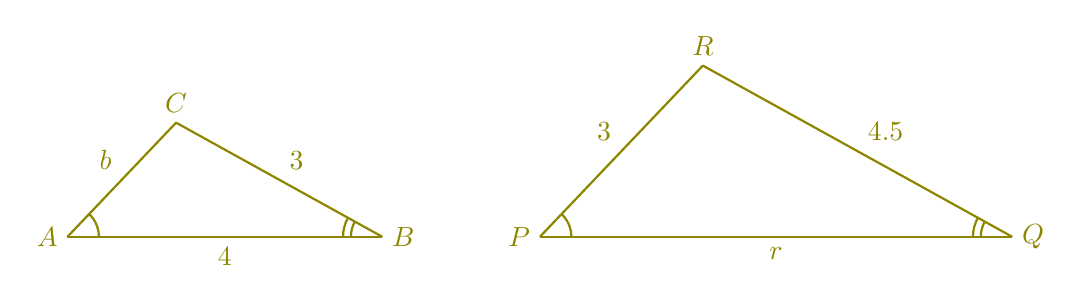
\begin{tikzpicture}
		\draw[color = olive, thick] (0,0) -- (4,0)
		node[midway, anchor = north] {$4$};
		\draw[color = olive, thick] (0,0) -- (1.38,1.45)
		node[midway, anchor = south east] {$b$};
		\draw[color = olive, thick] (1.38,1.45) -- (4,0)
		node[midway, anchor = south west] {$3$};
		\node[color = olive, anchor = east] at (0,0) {$A$};
		\node[color = olive, anchor = west] at (4,0) {$B$};
		\node[color = olive, anchor = south] at (1.38,1.45) {$C$};
		%VinkelA
		\draw[color = olive, thick] (0+0.4,0) arc (0:46.57:0.4); 
		%VinkelB
		\draw[color = olive, thick] (4-0.5,0) arc (180:180-28.96:0.5); 
		\draw[color = olive, thick] (4-0.4,0) arc (180:180-28.96:0.4); 
		%Trekant2
		\draw[color = olive, thick] (6,0) -- (12,0)
		node[midway, anchor = north] {$r$};
		\draw[color = olive, thick] (6,0) -- (1.38*1.5+6,1.45*1.5)
		node[midway, anchor = south east] {$3$};
		\draw[color = olive, thick] (1.38*1.5 + 6,1.45*1.5) -- (12,0)
		node[midway, anchor = south west] {$4.5$};
		\node[color = olive, anchor = east] at (6,0) {$P$};
		\node[color = olive, anchor = west] at (12,0) {$Q$};
		\node[color = olive, anchor = south] at (1.38*1.5 + 6,1.45*1.5) {$R$};
		%VinkelA
		\draw[color = olive, thick] (6+0.4,0) arc (0:46.57:0.4); 
		%VinkelB
		\draw[color = olive, thick] (12-0.5,0) arc (180:180-28.96:0.5); 
		\draw[color = olive, thick] (12-0.4,0) arc (180:180-28.96:0.4);		
		\end{tikzpicture}
	\caption{Eksempel på ensvinklede trekanter}
	\label{fig:ensvinkledeExa}
	\end{figure}
	Siderne $a = 3$ og $p = 4.5$ giver os størrelsesforholdet mellem disse trekanter. Dette tal betegnes typisk 
	med $k$ og kaldes \textit{skalafaktoren}. Skalafaktoren skal opfylde, at $k\cdot 3 = 4.5$. Derfor må 
	$k = 1.5$. Vi kan bruge skalafaktoren til at bestemme længden på de resterende linjestykker. For $r$ må der 
	gælde, at 
	\begin{align*}
		r = 4\cdot 1.5 = 6,
	\end{align*}
	og for $b$ må der gælde, at 
	\begin{align*}
		1.5\cdot b = 3 \ \Leftrightarrow \ b = \frac{3}{1.5} = 2.
	\end{align*}
\end{exa}	
Af eksemplet kan vi altså se, at skalafaktoren kan bruges til at bestemme sidelængder i ensvinklede trekanter. Dette fremgår også af følgende sætning.
\begin{setn}[Ensvinklede trekanter]
	For ensvinklede trekanter gælder der, at forholdet mellem siderne er parvist konstant. Med udgangspunkt i 
	Figur \ref{fig:ensvinklede} gælder der mere præcist for trekanterne $\triangle ABC$ og $\triangle PQR$, at
	\begin{align*}
		\frac{p}{a} = \frac{q}{b} = \frac{r}{c} = k.
	\end{align*}
	Tallet $k$ kaldes for \textit{skalafaktoren} mellem $\triangle ABC$ og $\triangle PQR$.
\end{setn}

\section*{Arealer af trekanter}

Vi fortsætter med at genopfriske formler og begreber fra grundskolen, og vi skal her gense formlen for arealet for en trekant. Vi betragter trekanterne på Figur \ref{fig:areal}
\begin{figure}[H]
	\centering
	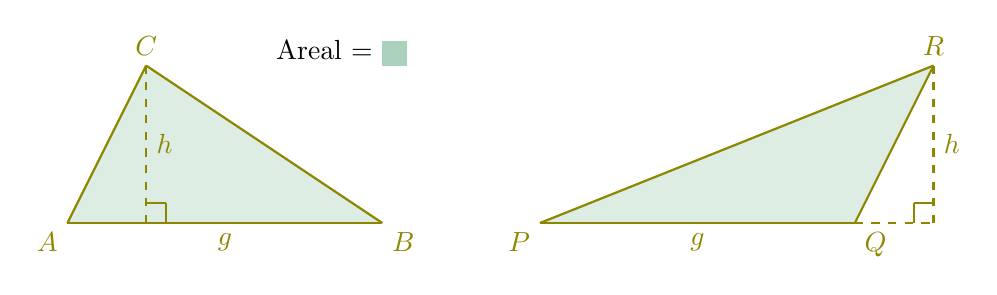
\begin{tikzpicture}
	%Trekant1
	\coordinate (1) at (0,0);
	\coordinate (2) at (4,0);
	\coordinate (3) at (1,2);
	\fill[SeaGreen!40, opacity = 0.4] (1) -- (2) -- (3) -- cycle;
	\draw[color = olive, thick] (1) -- (2)
	node[midway, anchor = north] {$g$};
	\draw[color = olive, thick] (1) -- (3);
	\draw[color = olive, thick] (2) -- (3);
	\node[color = olive, anchor = north east] at (1) {$A$};
	\node[color = olive, anchor = north west] at (2) {$B$};
	\node[color = olive, anchor = south] at (3) {$C$};
	\draw[color = olive, dashed, thick] (1,0) -- (1,2)
	node[midway,anchor = west] {$h$};
	\draw[color = olive, thick] (1,0.25) -- (1.25,0.25);
	\draw[color = olive, thick] (1.25,0) -- (1.25,0.25);
	\filldraw[color = SeaGreen!40] (4,2) rectangle (4.3,2.3);
	\node[anchor = east] at (4,2.2) {Areal = };
	
	 
	%Trekant2
	\coordinate (4) at (6,0);
	\coordinate (5) at (10,0);
	\coordinate (6) at (11,2);
	\fill[SeaGreen!40, opacity = 0.4] (4) -- (5) -- (6) -- cycle;
	\draw[color = olive, thick] (4) -- (5)
	node[midway, anchor = north] {$g$};
	\draw[color = olive, thick] (4) -- (6);
	\draw[color = olive, thick] (5) -- (6);
	\node[color = olive, anchor = north east] at (4) {$P$};
	\node[color = olive, anchor = north west] at (5) {$Q$};
	\node[color = olive, anchor = south] at (6) {$R$};
	\draw[color = olive, dashed, thick] (11,0) -- (11,2)
	node[midway,anchor = west] {$h$};
	\draw[color = olive, dashed, thick] (10,0) -- (11,0);
	\draw[color = olive, thick] (10.75,0.00) -- (10.75,0.25);
	\draw[color = olive, thick] (10.75,0.25) -- (11,0.25);
	\end{tikzpicture}
	\caption{Areal for trekanter samt højde og grundlinje}
	\label{fig:areal}
\end{figure}
\newpage
\begin{setn}[Areal af trekant]
	Arealet $M$ for en trekant $\triangle ABC$ med højde $h$ og grundlinje $g$ som set på Figur \ref{fig:areal} 
	er givet ved
	\begin{align*}
		M = \frac{1}{2}\cdot h \cdot g.
	\end{align*}
\end{setn}
\begin{exa}
En trekant $\triangle ABC$ er givet på Figur \ref{fig:arealExa}.
\begin{figure}[H]
	\centering
	\begin{tikzpicture}
	\coordinate (1) at (0,0);
	\coordinate (2) at (6,0);
	\coordinate (3) at (1,4);
	\draw[color = olive, thick] (1) -- (2)
	node[midway, anchor = north] {$6$};
	\draw[color = olive, thick] (1) -- (3);
	\draw[color = olive, thick] (2) -- (3);
	\node[color = olive, anchor = north east] at (1) {$A$};
	\node[color = olive, anchor = north west] at (2) {$B$};
	\node[color = olive, anchor = south] at (3) {$C$};
	\draw[color = olive, dashed, thick] (1,0) -- (1,4)
	node[midway,anchor = west] {$4$};
	\draw[color = olive, thick] (1,0.25) -- (1.25,0.25);
	\draw[color = olive, thick] (1.25,0) -- (1.25,0.25);
	\end{tikzpicture}
	\caption{Trekant med højde og grundlinje angivet.}
	\label{fig:arealExa}
\end{figure}
Vi kan på figuren aflæse, at højden $h = 4$ og grundlinjen $g = 6$. Vi udregner arealet $M$ af trekanten og får
\begin{align*}
	M = \frac{1}{2}\cdot 4 \cdot 6 = 12.
\end{align*} 
\end{exa}

\subsection*{Opgave 1}
En trekant $\triangle ABC$ er givet som følgende
\begin{center}
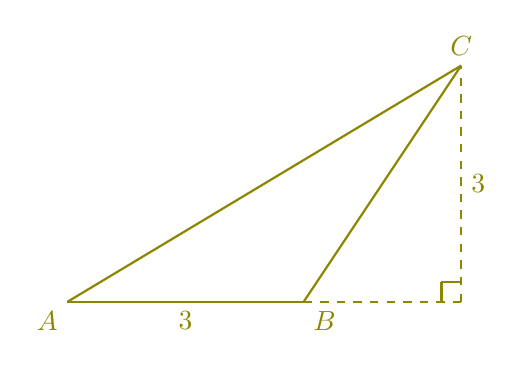
\begin{tikzpicture}
	\coordinate (1) at (0,0);
	\coordinate (2) at (3,0);
	\coordinate (3) at (5,3);
	\draw[color = olive, thick] (1) -- (2)
	node[midway, anchor = north] {$3$};
	\draw[color = olive, thick] (1) -- (3);
	\draw[color = olive, thick] (2) -- (3);
	\node[color = olive, anchor = north east] at (1) {$A$};
	\node[color = olive, anchor = north west] at (2) {$B$};
	\node[color = olive, anchor = south] at (3) {$C$};
	\draw[color = olive, dashed, thick] (5,0) -- (5,3)
	node[midway,anchor = west] {$3$};
	\draw[color = olive, thick] (4.75,0) -- (4.75,0.25);
	\draw[color = olive, thick] (4.75,0.25) -- (5,0.25);
	\draw[color = olive, thick, dashed] (3,0) -- (5,0);
\end{tikzpicture}
\end{center}
\begin{enumerate}[label=\roman*)]
	\item Bestem arealet af trekanten. 
\end{enumerate}
\subsection*{Opgave 2}
En trekant har højde $5$ og areal $10$. 
\begin{enumerate}[label=\roman*)]
	\item Bestem længden af grundlinjen for trekanten. 
\end{enumerate}

\subsection*{Opgave 3}
To trekanter $\triangle ABC$ og $\triangle PQR$ er givet ved
\begin{center}
\begin{tikzpicture}
	%Trekant1
	\coordinate (1) at (0,0);
	\coordinate (2) at (3,0);
	\coordinate (3) at (3.5,1.94);
	\draw[color = olive, thick] (1) -- (2)
	node[midway, anchor = north] {$3$};
	\draw[color = olive, thick] (1) -- (3)
	node[midway, anchor = south east] {$4$};
	\draw[color = olive, thick] (2) -- (3)
	node[midway, anchor = north west] {$a$};
	\node[color = olive, anchor = north east] at (1) {$A$};
	\node[color = olive, anchor = north west] at (2) {$B$};
	\node[color = olive, anchor = south] at (3) {$C$};
	\draw[color = olive, thick] (0+0.5,0) arc (0:28.96:0.5);
	\draw[color = olive, thick] (3-0.4,0) arc (180:180-104.48:0.4);
	\draw[color = olive, thick] (3-0.5,0) arc (180:180-104.48:0.5);
	 
	%Trekant2
	\coordinate (4) at (0+5,0);
	\coordinate (5) at (3*2+5,0);
	\coordinate (6) at (3.5*2 + 5,1.94*2);
	\draw[color = olive, thick] (4) -- (5)
	node[midway, anchor = north] {$r$};
	\draw[color = olive, thick] (4) -- (6)
	node[midway, anchor = south east] {$8$};
	\draw[color = olive, thick] (5) -- (6)
	node[midway, anchor = north west] {$4$};
	\node[color = olive, anchor = north east] at (4) {$P$};
	\node[color = olive, anchor = north west] at (5) {$Q$};
	\node[color = olive, anchor = south] at (6) {$R$};
	\draw[color = olive, thick] (0+0.5+5,0) arc (0:28.96:0.5);
	\draw[color = olive, thick] (3*2-0.4+5,0) arc (180:180-104.48:0.4);
	\draw[color = olive, thick] (3*2-0.5+5,0) arc (180:180-104.48:0.5);
	\end{tikzpicture}
\end{center}
\begin{enumerate}[label=\roman*)]
	\item Bestem skalafaktoren $k$ samt længden af siderne $a$ og $r$.
\end{enumerate}

\subsection*{Opgave 4}
To ensvinklede trekanter $\triangle ABC$ og $\triangle PQR$ har sidelængderne $a = 5$, $b = 7$, $q = 17.5$ og $r = 10$.
\begin{enumerate}[label=\roman*)]
	\item Tegn en skitse af de to trekanter. 
	\item Bestem skalafaktoren for de to trekanter og brug denne til at bestemme de ukendte sider i trekanten
\end{enumerate}

\subsection*{Opgave 5}
To trekanter $\triangle ABC$ og $\triangle PQR$ er givet ved følgende figur. Det oplyses desuden, at arealet af 
$\triangle ABC$ er lig 6 samt at arealet af $\triangle PQR$ er lig $24$. 


\begin{center}
\begin{tikzpicture}
	%Trekant1
	\coordinate (1) at (0,0);
	\coordinate (2) at (4,0);
	\coordinate (3) at (0,3);
	\draw[color = olive, thick] (1) -- (2)
	node[midway, anchor = north] {$c$};
	\draw[color = olive, thick] (1) -- (3)
	node[midway, anchor = east] {$3$};
	\draw[color = olive, thick] (2) -- (3)
	node[midway, anchor = south west] {$a$};
	\node[color = olive, anchor = north east] at (1) {$A$};
	\node[color = olive, anchor = north] at (2) {$B$};
	\node[color = olive, anchor = south] at (3) {$C$};
	\draw[color = olive, thick] (4-0.5,0) arc (180:180-36.87:0.5);
	\draw[color = olive, thick] (0.25,0) -- (0.25,0.25);
	\draw[color = olive, thick] (0,0.25) -- (0.25,0.25);
	
	 
	%Trekant2
	\coordinate (4) at (0+5,0);
	\coordinate (5) at (8+5,0);
	\coordinate (6) at (5,6);
	\draw[color = olive, thick] (4) -- (5)
	node[midway, anchor = north] {$r$};
	\draw[color = olive, thick] (4) -- (6)
	node[midway, anchor = east] {$q$};
	\draw[color = olive, thick] (5) -- (6)
	node[midway, anchor = south west] {$p$};
	\node[color = olive, anchor = north] at (4) {$P$};
	\node[color = olive, anchor = north west] at (5) {$Q$};
	\node[color = olive, anchor = south] at (6) {$R$};
	\draw[color = olive, thick] (-0.5+13,0) arc (180:180-36.87:0.5);
	\draw[color = olive, thick] (0.25+5,0) -- (0.25+5,0.25);
	\draw[color = olive, thick] (0+5,0.25) -- (0.25+5,0.25);
	\end{tikzpicture}
\end{center}

\begin{enumerate}[label=\roman*)]
	\item Bestem tallet $c$.
	\item Bestem skalafaktoren for trekanterne. (Vink: udnyt, at $q = bk$ og $r = ck$ og indsæt i arealformlen)
	\item Bestem tallene $q$ og $r$. 
	\item Kan du huske, hvordan man bestemmer tallene $a$ og $p$?
\end{enumerate}

\subsection*{Opgave 6}

Vi skal måle højden på et eller andet højt ved brug af ensvinklede trekanter og et målebånd. 
\begin{enumerate}[label=\roman*)]
	\item Find noget højt. 
	\item Brug hvad i ved om ensvinklede trekanter samt et målebånd til at bestemme højden. 
\end{enumerate}

\subsection*{Opgave 7}
Om to ensvinklede trekanter $\triangle ABC$ og $\triangle AQR$ gælder det, at $|AB| = 4$ og $|BQ| = 3$ samt at højden af $\triangle AQR$ er $5.25$. 
\begin{center}
	\begin{tikzpicture}
	\coordinate (1) at (0,0);
	\coordinate (2) at (4,0);
	\coordinate (3) at (2.5,3);
	\draw[color = olive, thick] (1) -- (2);
	\draw[color = olive, thick] (1) -- (3);
	\draw[color = olive, thick] (2) -- (3);
	\node[color = olive, anchor = north east] at (1) {$A$};
	\node[color = olive, anchor = north] at (2) {$B$};
	\node[color = olive, anchor = south] at (3) {$C$};
	%Trekant2
	\coordinate (4) at (0,0);
	\coordinate (5) at (7,0);
	\coordinate (6) at (1.75*2.5,1.75*3);
	\draw[color = olive, thick] (4) -- (5);
	\draw[color = olive, thick] (4) -- (6);
	\draw[color = olive, thick] (5) -- (6);
	\node[color = olive, anchor = north west] at (5) {$Q$};
	\node[color = olive, anchor = south] at (6) {$R$};
	\end{tikzpicture}
\end{center}
\begin{enumerate}[label=\roman*)]
	\item Bestem arealet af $\triangle ABC$.
\end{enumerate}
